\subsubsubsubsection{Bicycle}
\begin{figure}[h]
\centering
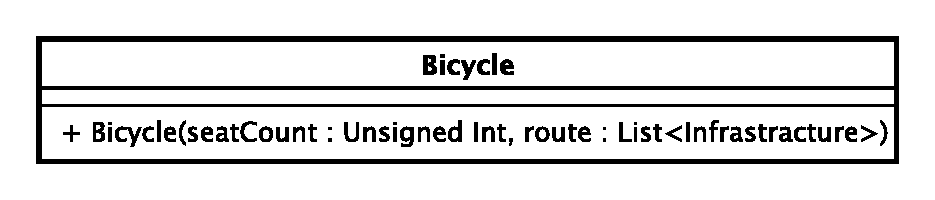
\includegraphics[scale=0.6,keepaspectratio]{images/solution/app/backend/bicycle.eps}
\caption{\pActive::Bicycle}
\label{fig:sd-app-bicycle}
\end{figure}
\FloatBarrier
\begin{itemize}
  \item \textbf{\descr} \\
It represents a urban traveller that moves only on bikepaths.
  \item \textbf{\ops}
  \begin{itemize}
  \item[+] \texttt{Bicycle(seatCount : Unsigned Int, route : List<Infrastructure>)} \\
Creates a bicyle specifying its number of seats.
  \end{itemize}
\end{itemize} 
